\documentclass{llncs}

\usepackage[slovak]{babel}
\usepackage[IL2]{fontenc}
\usepackage[utf8]{inputenc}
%Prvé tri balíčky zaisťujú správne vypisovanie slovenských znakov v dokumente 
\usepackage{graphicx}
%Tento balíček umožňuje pracovať s grafikou, konkrétne s obrázkami
\usepackage{fancyhdr}
%Fancyhdr dovolí užívateľovi používať príkazy na zmenu organizácie strán. V mojom prípade som menil hlavičku, lebo nebola definovaná v šablóne
\pagestyle{fancy}
%Príkaz pre kt. je potrebný balíček fancyhdr a nastavuje štýl strany na vlastný
\fancyhead[LE]{\thepage  \hspace{25pt}      Holub, M., Proksa, O., Bieliková, M.}
\fancyhead[RO]{Detecting Identical Entities in the Semantic Web Datas  \hspace{25pt} \thepage}
%2 príkazy ktoré konkrétne menia hlavičky strán. [LE]bude hlavičku písať na ľavú stranu párnych strán a [RO] na pravú stranu nepárnych strán. thepage vypíše číslo strany a hspace urobí medzeru veľkosti 25 bodov 
\renewcommand{\headrulewidth}{0pt}
%Príkaz kt. odstráni podčiarknutie hlavičiek strán
\newcommand\tab[1][0.5cm]{\hspace*{#1}}
% Tento príkaz mení prednastavenú veľkosť medzier v príaze tab 
\begin{document}
\title{Detecting Identical Entities in the Semantic Web Data}

\author{Michal Holub, Ondrej Proksa, and Mária Bieliková}

\institute{Institute of Informatics and Software Engineering\\Faculty of Informatics and Information Technologies, Slovak University of Technology,\\
 Ilkovičova 2, 842 16, Bratislava, Slovakia\\
\email{michal.holub@stuba.sk,ondrej.proksa@gmail.com,maria.bielikova@stuba.sk},
}

\maketitle            

\begin{abstract}
Large amount of entities published by various sources inevitably
introduces inaccuracies, mainly duplicated information. These
can even be found within a single dataset. In this paper we propose
a method for automatic discovery of identity relationship between two
entities (also known as instance matching) in a dataset represented as
a graph (e.g. in the Linked Data Cloud). Our method can be used for
cleaning existing datasets from duplicates, validating of existing identity
relationships between entities within a dataset, or for connecting different
datasets using the owl:sameAs relationship. Our method is based on the
analysis of sub-graphs formed by entities, their properties and existing
relationships between them. It can learn a common similarity threshold
for particular dataset, so it is adaptable to its different properties. We
evaluated our method by conducting several experiments on data from
the domains of public administration and digital libraries.
\vspace{5mm} \\
% vspace urobí 5cm medzeru po dopísanom riadku a v kombinácii s dvojitým backslashom sa najbližší riadok bude vypisovať od začiatku (bez tabolátora)
\textbf {Keywords:} duplicates, identity, similarity, relationship, Semantic Web,
owl:sameAs, Linked Data, Web of Data
\end{abstract}

\section{Introducion}

The Web has shifted from a group of pages into an interconnected network of
information processable by automatic agents. Many web pages contain struc-
tured data in formats such as XML or RDFa. New methods for extracting struc-
tured information from unstructured data emerge \cite{auer2007dbpedia,suchanek2007yago}. Facts about real-world
entities are grouped into various datasets and published on the Web. More-
over, datasets are connected with each other using links and shared vocabularies
(schemas), thus forming the Linked Data Cloud.

These datasets have the form of graphs with vertices representing entities
and values, and edges representing relationships. They capture semantics usable
for various adaptation and personalization tasks. Linked Data can help with
content-based recommendations, answering near natural language search queries,
filtering relevant information, or adapting web pages to specic users.

Linked Data can also be used in detection of similarity between objects,
relationship discovery, or semantic enrichment of existing web pages. For all these
tasks we need to have a good representation \cite{harth2012database}.
The main problem linked with
representation is the discovery of similarity and identity between entities \cite{weikum2010information}.

An imminent problem of large datasets is that they usually contain duplicates
and it is a challenge to find them. This is also referred to as the data linking
problem where the goal is to find equivalent resources on the Semantic Web \cite{daskalaki2014instance}.

Marking entities as duplicates on the Semantic Web is usually done using a
owl:sameAs relationship. However, a study \cite{halpin2010owl} proved, that owl:sameAs is often
wrongly used to connect e.g. two people or other objects with identical names,
although their other attributes are not identical and they represent diferent real-
world entities. Another problem is that sometimes owl:sameAs is deliberately or
mistakenly used to connect very similar, although not identical entities.

In this paper we address the problem of identifying if two entities are the same
with satisfactory precision. Our main goal is to discover whether two entities in
one dataset refer to the identical real-world object, a problem which is also
known as instance matching. We use graph algorithms and specific rules on
various attributes, results of which we combine in a specific way tailored for
each dataset in order to determine if two given entities are the same.

In our experiments we focused on finding duplicate people and companies
in various datasets. Our main contribution is that the proposed method can
automatically adapt to varying properties of datasets.

\section{Related work}

Because the Linked Data datasets use various ontologies and schemas to describe
their content, there is a problem of ontology diversity, which could cause that
identical entities are not connected. Graph algorithms are used to address this
problem in \cite{zhao2012graph}. Graph patterns in the form of sub-graphs with identical vertices
and edges are defined. At first, the authors integrate two datasets and detect the
graph patterns in them. Then, ontology alignment on each of the graph patterns
is performed. Finally, it aggregates similar ontology classes and properties.

Detecting duplicates in XML data was examined in \cite{leitao2013efficient}.. The authors proposed
to combine not only the information within elements, but also the information
about how the data is structured. Their solution uses Bayesian network to de-
termine the degree of similarity of two entities.

Analyzing sub-graphs of compared entities is also used in the domain of on-
tology matching problem \cite{aumueller2005schema,shvaiko2013ontology}. They usually compare two similar datasets (de-
scribing the same domain, very similar entities and relationships but described
using different schemas with different names). The prior knowledge that the two
compared datasets are very close to each other makes the comparison easier,
unless we are comparing one very rich dataset (lots of entities with plethora of
attributes, richly connected through various relationships) with very sparse one
(only few entities' attributes and basic relationships).

This approach can be used to map more ontologies to each other, and thus
discovering identical entities in datasets which use these ontologies. 
this approach is that it requires manual verification as the precision is not high
enough. This can be diffcult and time consuming, especially for large datasets.

Another approach using graph algorithms is described in \cite{lehmann2007discovering}. The proposed
method finds relationships among entities in DBpedia. Its main idea is to split
the graph into its components using the breadth-first search. Then, the shortest
path between two entities is computed. The disadvantage is not considering the
type of the relationship. However, we can use the presence of such relationship
as an indicator that the two entities are identical.

When performing the instance matching the usual approach is to 1) quickly
scan the whole dataset to find entities for comparison, and 2) measure the sim-
ilarity between pairs of entities found in the previous step \cite{volz2009silk,ngomo2011limes}.

This approach is also used in \cite{araujo2012serimi}. The authors propose a method for instance
matching using class hierarchy of instances. For selecting candidates of poten-
tially identical entities they use small number of characteristic attributes (e.g.
name or title). Then they search for entities which have similar values of these
attributes. The challenge here is automatic selection of characteristic attributes,
as well as the similarity threshold for the values of attributes.

Selecting potential candidates allows the algorithm to scale on large datasets.
Otherwise, we would have to compare each possible pair of entities, resulting
in quadratic complexity. On the other hand, if this step is executed with low
precision, we may omit some duplicates, so on smaller datasets it is desirable to
compare as many pairs of entities as possible.

A suitable similarity measure has to be applied on the attributes of com-
pared entities. Each pair of attributes can be compared using different similarity
measure according to the data type, e.g. text or numeric similarity. There can
also be more complex measures, comparing e.g. geo data or address records [15].
We need to know the semantics of the attributes to correctly select the metrics.

Current approaches use either attribute values to compare pairs of enti-
ties \cite{nikolov2012unsupervised}, or graph algorithms to compute the similarity based on entity's re-
lationships with its neighbors \cite{melnik2002similarity}. Instances can also be matched based on the
representation of their metadata \cite{shvaiko2005survey}. However, various datasets need different
approaches according to their properties. In many datasets it is vital to use a
combination of approaches with weights tailored for a particular domain.

\section{Detecting similarity between entities}

We propose a method for finding if two given entities are identical. It can compare
each pair of entities within a dataset (or possibly more datasets). The method
was designed to work on datasets which can be represented using graphs, such
as (but not limited to) RDF representation, the basis of the Linked Data Cloud.

Our method is based on a hypothesis that the matching of entities is reflected
in the similarity between the sub-graphs composed of classes and properties of
the individual entities. For a given pair of entities we compute how similar they
are. Then, we determine a common similarity threshold, above which we mark
the entities to be identical.

We use matching of features of entities, as well as properties of the sub-
graphs they are part of. Our method computes the similarity between entities as
a weighted sum of these four partial parameters: 1) similarity of entities' proper-
ties, 2) graph distance between entities, 3) graph distance between neighboring
entities, and 4) similarity of entities' relationships:

\begin {equation}
SGN=\frac{SNP\times w_{SNP}+SNR\times w_{SNR}+ND \cdot  w_{ND}+DRN\times w_{DRN}}{w_{SNP} + w_{SNR} + w_{ND} + w_{DRN}}
%times urobí exponent v rovnici a cdot urobí skalárny súčin
\label{rov1}
\end {equation}
where
\newline
SGN - similarity of graph nodes, final similarity between two entities\\
SNP - similarity of entities' properties\\
SNR - similarity of relationships between entities\\
ND - graph distance between entities\\
DRN - average graph distance between adjacent entities\\
$w_i$ - weight of a particular component\\
\vspace{5mm} \\
The resulting values of the similarity, as well as the results produced by each
component, are from the interval [0, 1]. Similarity = 1:0 means that the two
entities are 100\%  similar (i.e. identical), whereas similarity = 0:0 means that the
two entities are not similar at all. All components of the eq. 1 have associated
weights, which determine the component's contribution to the total similarity.

In some datasets (e.g. in the domain of public administration data) it turns
out that the entities' properties are more important than relationships between
them (the records contain a lot of attributes, but few connections). On the other
hand, in domains such as social networks or digital libraries, there are many
relationships between entities, so the weights of related similarity components
should be higher. In our approach the weights can be automatically trained, so
that our method can adapt itself to a particular problem domain. They can also
be assigned manually by a domain expert.

As we already mentioned, we compute the similarity of two entities A;B from
the interval $SGN_{A,B} \in [0, 1]$. To determine whether these entities are identical
we need to find a threshold of similarity (denoted S) from the same interval.
The threshold S should be determined for each domain differently, as it should
reflect dataset's properties.

\subsection{Similarity of properties between entities (SNP)}
When computing the similarity of properties (attributes) of two entities, we need
to use suitable similarity measure according to the data types used. This is illustrated in Tab.
\ref{tab1} representing people in a dataset of owners of companies in
Slovakia, which provides example properties used when comparing two entities.
As we can see, not all types of properties can be compared using textual similar-
ity. Example in the first row depicts that sometimes the attribute labelled name
contains not only the name of a person (entity A), but also an abbreviation of
related organization (entity B). Row 2 demonstrates that names and addresses
may be mixed together.

\begin{table}
\centering
\renewcommand\tablename{Table}
\caption{Comparison of example properties between various pairs of entities.}
\label{tab1}
\begin{tabular}{|c|c|c|c|l|}
\hline
Property label &  & Entity A    & \multicolumn{2}{c|}{Entity B}     \\ \hline
Name   &  & Jozef Turanovsky      & \multicolumn{2}{c|}{Jozef Turanovsky - UNIP}    \\ \hline
Name, Address  &  & \begin{tabular}[c]{@{}c@{}}Juraj Siroky\\ Strme vrsky 137\end{tabular}    & \multicolumn{2}{c|}{\begin{tabular}[c]{@{}c@{}}Mgr. Juraj Siroky 137\\ Strmy vrsok 137\end{tabular}} \\ \hline
Address    &  & \begin{tabular}[c]{@{}c@{}}Zombova 19 \\ 040 23 Kosice - Sidlisko KVP\end{tabular} & \multicolumn{2}{c|}{\begin{tabular}[c]{@{}c@{}}Lomonosovova 30\\  040 01 Kosice - Juh\end{tabular}}  \\ \hline
District       &  & Kosice II  & \multicolumn{2}{c|}{Kosice 4}     \\ \hline
\end{tabular}
\end{table}
If the entities are in the same dataset (which is the primary concern of this paper)
or if their properties are described using the same vocabulary (ontology) we can
easily determine which properties to compare. Otherwise, we need to apply some
matching algorithm to determine appropriate attributes for comparison. For the
similarity of properties between entities A and B we define:\\
$PR_x$ =\{$prop_1$, $ prop_2$, ...$ prop_n$\} - denotes a set of properties of entity x\\
$PR_y$ = \{$prop_1$, $prop_2$, ... $prop_m$\} - denotes a set of properties of entity y\\
$PR_{x,y}$ =$ PR_x \cap PR_y$  - denotes a set of properties common to both entities x and y
\newline
Similarity of properties (sig. SNP) between entities is defined as follows:
\begin {equation}
SNP=\frac{SP_0 \times w_{P0} +SP_1 \times w_{P1} + ... +SP_k \times w_{Pk}}{w_{P0} + w_{P1} + ... + w_{Pk}}
\label{rov2}
\end {equation}
\newline
where\\
$SP_0, SP_1,...,  SP_n$ - similarity between common properties (text, numeric, etc.)\\
$w_{P0} , w_{P1} ,...; w_{Pn}$ - weight of each similarity\\
\newline
Again, we determine the component's importance using weights which we train
using machine learning. The eq. \ref{rov2} reflects the weighted average of the individual
similarities between the properties. Sometimes, it is possible that some properties
will be ignored (we set their weight to zero).We do not consider properties unique
to some entity, only those common to both of the compared entities.

We compare the properties of entities using textual similarity and numerical
similarity. Textual similarity of properties is the average between the Levenshtein
distance and 3-gram similarity of the compared properties, as these metrics
are widely used and their good performance has been confirmed. Numerical
similarity is defined the normalized numerical distance, which we compute as
follows:

\begin{equation}
ndist(num_A, num_B)= \frac {MAX_{num} - |num_A - num_b|}{MAX_{num}}
\label{rov3}
\end{equation}
where\\
\vspace{5mm} \\
$ndist(num_A, num_B)$ - normalized distance between the numbers, $ ndis \in [0, 1]$
$MAX_{num}$ - maximum value of the numerical properties in the domain
\vspace{8mm} 
\newline
\textbf{Linking properties from different vocabularies}\newline
\vspace{1.5mm} \\
Existing approaches usually consider the fact that the entities are described
using the same vocabulary, so the names of properties will match. A problem
occurs when the properties are defined using different schemas.Tab. \ref{tab2} presents
a comparison of several names of properties in DBpedia and YAGO datasets. As
we can see, some of the names do not match, although they describe the same
fact. 
\begin{table}
\centering
\renewcommand\tablename{Table}
\caption{Comparison of names of equal properties between DBpedia and YAGO.}
\label{tab2}
\begin{tabular}{|l|l|l|}
\hline
\textbf{Property} & \textbf{Name in DBpedia} & \textbf{Name in YAGO}  \\ \hline
School            & \textit{almaMater}       & \textit{school}        \\ \hline
Date of birth     & \textit{birthDate}       & \textit{wasBornOnDate} \\ \hline
Nationality       & \textit{nationality}     & \textit{nationality}   \\ \hline
Place of birth    & \textit{birthPlace}      & \textit{wasBornIn}     \\ \hline
Title             & \textit{title}           & \textit{title}         \\ \hline
\end{tabular}
\end{table}
To solve this problem we also use semantic similarity of properties' names.\\
The semantic similarity between words is not easily computable as in general we
do not know exact meaning of the words. Also, we often do not have complete
information on their context. We use WordNet in order to determine if two words
are in the same synset. Once at least one of these similarities is above the given
threshold, we can say that the names represent the same property, so that we
can compare the values using previously described metrics.

In order to link the names of the properties we take all the properties of the
entity A. Then, we find the most similar property of the entity B according to its
name. When the entities come from different datasets, it is not always possible
to connect all the properties. Subsequently, we consider only the properties we
are able to link when computing the overall similarity of properties (SNP).

\subsection {Distance between the entities (ND)}
When calculating the distance between two entities in a graph we use the algo-
rithm of breadth-first search. Our intention is to find the shortest path between
the entities. We consider every edge to have the length of 1. The final distance
is normalized to the interval [0, 1]. Normalization is based on the minimum and
maximum distance in the given data set.

Maximum and minimum distances for the normalization must be set for each
data set separately in the preprocessing phase. We experimented in the domain of
public administration data, where the minimum distance between organizations
is at least 2. Also, we conducted experiments on data from digital libraries, where
the minimum and maximum distances between papers' authors are different (for
more details see evaluation).

\subsection {Average distance between adjacent entities (DRN)}
The average distance between the two entities is defined as the normalized aver-
age distance computed from the smallest distances to the neighboring entities.
We compute DRN of entities A and B using their direct neighbors (see Fig. 1).
In \ref{fig1} entity A has three neighboring entities -$ RN_{A1}, RNA_2 and RNA_3.$
Entity B has four neighboring entities -$ RN_{B1}, RNB_2, RNB_3 and RNB_4.$ For
each neighboring entity of A we find the closest neighboring entity of B and use
their distance. The value of DRN between A and B is equal to the average of
these distances. Finally, we normalize the average distance using maximum and
minimum average distances according to eq. 4.

\begin {equation}
DRN(A,B)=\frac{MAX_{drn}-avg\_dist(A, B)}{MAX_{drn}-MIN_{drn}}
\label{rov4}
\end{equation}

\begin {equation}
     avg\_dist(A,B)  =\frac {\Sigma \forall RN_{Bj} \in RN_B : min(RN{Ai},RN_{Bj})}{|RN_A|}
\label{rov5}
\end{equation}
where\newline
$DRN(A, B)$ - normalized average distance between $A and B, DRN(A B) \in [0, 1]$\\
$avg\_dist(A, B) $- average distance between entities $A and B$\\
$MIN_{drn}$ - minimum average distance between entities\\
$MAX_{drn}$ - maximum average distance between entities

\subsection{Similarity of relationships between entities (SRN)}
The last component of the similarity computation is the similarity of entities'
relationships. For both entities A and B we divide their neighboring entities
according to the type of the relationship between them. For each type we express
the Jaccard coefficient between sets of adjacent entities of A and adjacent entities
of B and we compute the average of the Jaccard coefficients:
\begin {equation}
SNR(A,B)=\frac {j(RNA_{R1},RNB_{R1})+...+j(RNA_{Rn},RNB_{Rn})}{|R|}
\end {equation}
where\newline
$R$ - list of the types of relationships for which the neighboring entities of $A$ and
$B$ form non-empty sets
$j(R_A R_B)$ - Jaccard coefficient between sets of neighboring entities of A and B
\begin{figure}
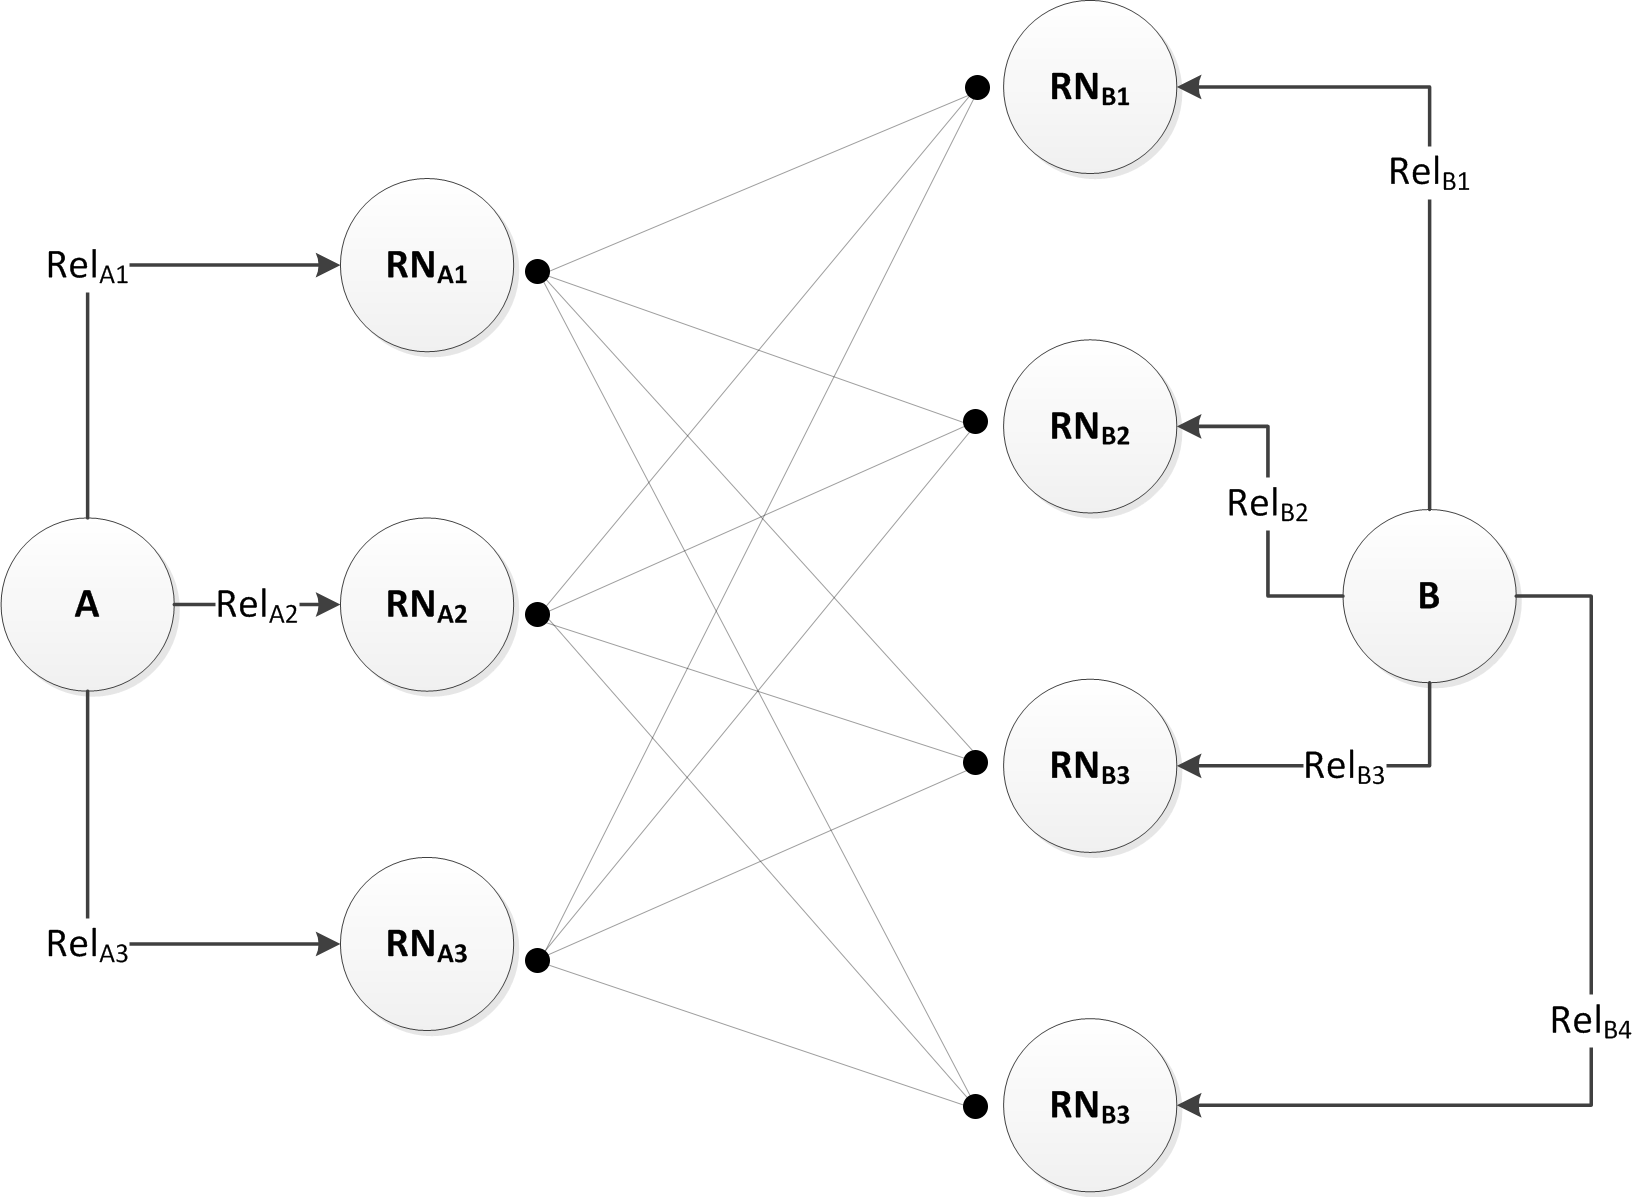
\includegraphics[width=1\linewidth]{OBR1.png}
\renewcommand\figurename{Fig}
\label {fig1}
\caption {Relationships nodes for two entities}
\end{figure}
\section{Evaluation}
We have conducted several experiments with various datasets in order to evaluate
specific parts of our method, from finding duplicate organizations to finding
namesakes of authors of research papers.

\subsection {Finding identical organizations}
In this experiment we used public data\footnote{http://naseobce.sk} with information about cities, villages,
regions and organizations in Slovakia. It contains a lot of duplicates and our goal
was to identify identical organizations which were wrongly labelled as diverse,
thus helping to clean the dataset.
%footnote urobí vysvetlivku na konci strany
Throughout the time, organizations may change their names, cease to exist
and be started again elsewhere, etc. However, each organization has assigned
its unique ID number, which persists event if the organization changes some
of its properties (e.g. name, owner). We used this ID for evaluation. For each
organization X we found two other organizations which we used to compute the
similarities: 1) one identical organization A with the same ID number, and 2)
one random organization B that has a different ID number.

We expected A to be the most similar organization to X and B to be the
least similar, according to our method. Note that have not used the unique ID
when computing the similarity, we only used it for selecting the entities and
evaluating the performance of our method.

For setting up the weights of components of our method we used machine
learning, particularly support vector machines.We trained on the 80\% and tested
on 20\% of the data. As a threshold (S) for two entities to be identical we used the
value of S = 0:5, which we set manually based on our observations of the available
data. This value could also be trained if enough test data was present. We used
precision, recall, accuracy and F1 score as standard metrics of performance.

The dataset used for this experiment was composed by a graph of 13,820
vertices, they had 119,484 properties and were connected using 131,683 relation-
ships. We compared the names and addresses of organizations. As a baseline we
used textual similarity computed using Levenshtein distance and 3-grams.

The results are summarized in Tab. \ref{tab3}. We used two setups: the first one
involved computing the SGN value using all similarity components, in the second
one we only computed the value of SNP (the similarity of properties). We have
performed the training and testing on 5,000 and 10,000 examples, respectively.

Using only the similarity of properties resulted in the best overall F1 score
because the entities' properties are the most dominant in this dataset. Including
other components has worsen the results. The baseline method was better when
finding identical organizations, but it also produced more false positives.

\begin{table}
\centering
\renewcommand\tablename{Table}
\caption{Results of experiment with identical organization identification.}
\label{tab3}
\begin{tabular}{|l|l|l|l|l|l|}
\hline
Method            & Size   & \textbf{Presicion} & \textbf{Recall} & \textbf{Accuracy} & \textbf{F1 score} \\ \hline
\textbf{SNP}      & 5,000  & 0.98981            & 0.98812         & 0.99014           & 0.99012           \\ \hline
\textbf{SNP}      & 10,000 & 0.99240            & 0.99275         & 0.99257           & 0.99257           \\ \hline
\textbf{SGN}      & 5,000  & 0.95532            & 0.82688         & 0.89409           & 0.88647           \\ \hline
\textbf{SGN}      & 10,000 & 0.96147            & 0.93057         & 0.94663           & 0.94576           \\ \hline
\textbf{3gramLev} & 5,000  & 1.00000            & 0.22811         & 0.61405           & 0.37148           \\ \hline
\textbf{3gramLev} & 10,000 & 1.00000            & 0.19275         & 0.59637           & 0.32320           \\ \hline
\end{tabular}
\end{table}

\subsection {Finding namesakes of the authors in DBLP}
In the second experiment we used data from DBLP digital library \cite{ley2002dblp}. In this
dataset the authors are not represented as separate entities (e.g. using unique
identificators), but only using their full names. No other information is available.
It is not clear when two records represent the same person or they are namesakes.
In this experiment we used our method to identify identical and diverse authors.\newline
\tab For each author we found the number of his namesakes using these steps:\newline
 1. Set the threshold to S = 0:5, a value we manually chose for this experiment.\newline
 2. For all papers transform all its authors to new temporary authors. Each
\tab temporal author was assigned to only one paper he wrote.\newline
3. For each temporary author find an identical temporary author using our
\tab method. Merge found authors to one entity. Repeat until no further tempo-
\tab rary author could be merged.

In order to evaluate the results we created an application which showed
authors and their papers. We asked 5 researchers to combine the authors with
the same name into one entity if all records represented one physical person.
Thus, we obtained a golden standard for evaluation of our method. The manually
processed dataset contained information about 100 distinct authors from three
research communities, each author had his associated papers. The researchers
were from the same communities and thus were able to correctly assess the
authors. The number of papers varied from 3 to 20 papers per author.

For each of the 100 authors we found his namesakes analyzing the whole
DBLP dataset (containing more than 1,300,000 author records). We then eval-
uated the precision of our method based on the number of namesakes it found
compared with the expected number of namesakes. We normalized these values
to the interval [0, 1] and we calculated the weighted average, where the weights
are the numbers of publications for all namesakes of the author. Normalized
precision for one author was calculated using the normalization interval, where
the minimum value was the original number of namesakes, and the maximum
value was the total number of papers (because one author can be divided into
at most as many namesakes as the number of papers he wrote). This way we
obtained the weighted mean precision of 96.35\%.

We compared our results with a method based on detecting communities
of authors according to co-authorship of research papers \cite{zaiane2009mining}. It assumes that
researchers who authored papers together are always the same people. How-
ever, author and his namesake would probably not have a common colleague, so
their publications and co-authors will form two separate clusters. Our method
outperformed this baseline by 12\%.

We also compared the number of namesakes our method found with the num-
ber from the golden standard. We derived the precision as the ratio of correctly
computed counts of namesakes to the number of all authors. Here, our result
was 80.2\%, whereas the baseline method achieved only 66.34\%.

It turns out that considering only co-authors and shared publications is not
always the best indicator for namesake detection. Our method achieved better
results because it combines graph patterns better representing the real situation.

\section {Conclusion}

We proposed a method for identifying duplicates in existing data and finding
identity relations between entities. It can be used to clean a dataset as well as to
verify existing relationships denoting duplicate entities (e.g. using owl:sameAs
link). Since we are able to process any graph data, our method can also be
applied on the Linked Data datasets.

Our method is proposed as universal, its main contribution is combining sim-
ilarity of attributes with the similarity of sub-graph neighbourhoods of compared
entities. This can be helpful when finding e.g. namesakes of a person according
to various other objects he is linked to. The method can automatically adapt its
components (using weights) to reflect the properties of a particular dataset.

One important step in our method is setting the similarity threshold (S)
which influences the accuracy. When the threshold is set too low it will result
Detecting Identical Entities in the Semantic Web Data 11
in high recall but low precision. Otherwise, setting the threshold too high will
produce high precision but very low recall.

We analyzed this on a dataset from the project Annota \cite{holub2014annota}, which is a social
bookmarking and annotation tool. It is primarily aimed at bookmarking research
papers available on the Web (with special support of metadata extraction from
digital libraries such as ACM DL\footnote{http://dl.acm.org}). Annota's RDF dataset contains over 71,000
research papers, 390,000 authors, 9,000 publications and 6,400 publishers.

For each author we randomly chose 5 other authors thus forming candi-
date pairs for duplicates. For each pair we calculated their similarity using our
method. We observed that when setting the threshold S < 0:5 we found dupli-
cates in around 70\% of the cases. When the threshold was S = 0:5 the share
of duplicates fell to around 32\% and setting the threshold to S = 0:6 resulted
in only around 2\% of duplicates. Because for each author we selected very few
candidates compared to all authors in the dataset, the probability of choosing
real duplicate was insignificantly small.

This feature can be used to automatically adjust the threshold for an un-
known dataset: randomly pair each entity with a small set of other entities, then
calculate the similarity between each pair of entities. Start with a low similarity
threshold and increment it iteratively until the number of duplicates found is
close to zero. For very large datasets this process should be performed only on
their subsets for performance sake.

The applications of our method are multiple: 1) it can be used to find dupli-
cates in an existing dataset in order to clean the data, 2) it can be used to verify
the existing identity relations, and 3) it can be used in the process of creating a
new dataset so that we do not include the same entities twice.

Our method could also be used to connect a newly created dataset to the
Linked Data cloud, which is vital for enriching the Semantic Web. Entities
marked as identical can be connected using owl:sameAs link. In the future work
we plan to evaluate this in experiments by linking Annota dataset to existing
RDF datasets available on the Web.
\newline
\newline
\textbf{Acknowledgement.} This work was partially supported by grants No. VG
1/0646/15 and APVV-0208-10.
 
\bibliographystyle{abbrv}
\bibliography{Referencie}
\end{document}
